\chapter{System Requirements}
\label{ch:system_requirements}

\section{External Interface Requirements}
This section describes the interfaces between the system and its external entities.

\subsection{User Interfaces}
The user interface should be intuitive and user-friendly. Below is a mockup example:

\begin{figure}[h]
    \centering
    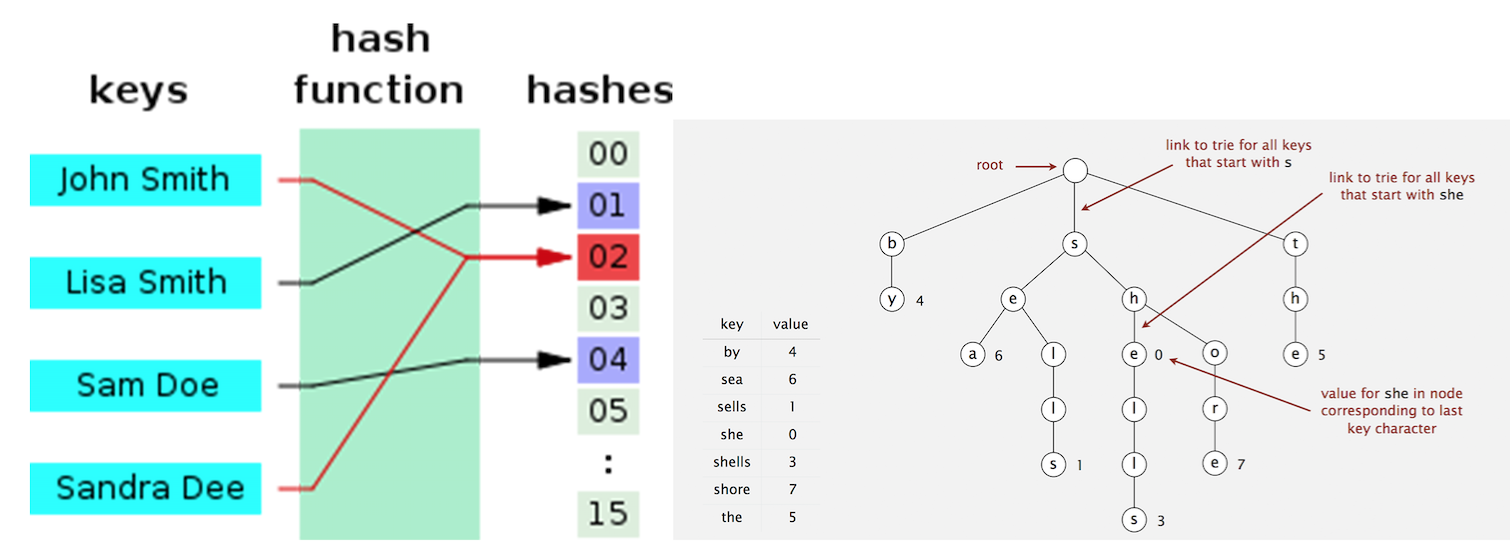
\includegraphics[width=0.8\textwidth]{images/hashing.png}
    \caption{Example User Interface Mockup}
    \label{fig:ui_mockup}
\end{figure}

\subsection{Hardware Interfaces}
The system interfaces with various hardware components, such as sensors and servers. Table~\ref{tab:hardware_interfaces} lists the hardware requirements.

\begin{table}[h]
    \centering
    \begin{tabular}{|l|l|l|}
        \hline
        \textbf{Hardware Component} & \textbf{Specification} & \textbf{Purpose} \\ \hline
        Sensor A & 1080p Resolution & Capturing data \\ \hline
        Server X & 16-Core CPU, 64GB RAM & Data processing \\ \hline
        Display Monitor & 1920x1080 Resolution & User interface \\ \hline
    \end{tabular}
    \caption{Hardware Interfaces}
    \label{tab:hardware_interfaces}
\end{table}

\subsection{Software Interfaces}
The required software interfaces include third-party libraries, APIs, and other software systems that interact with the product. Figure~\ref{fig:software_architecture} provides an overview of the software architecture.

\begin{figure}[h]
    \centering
    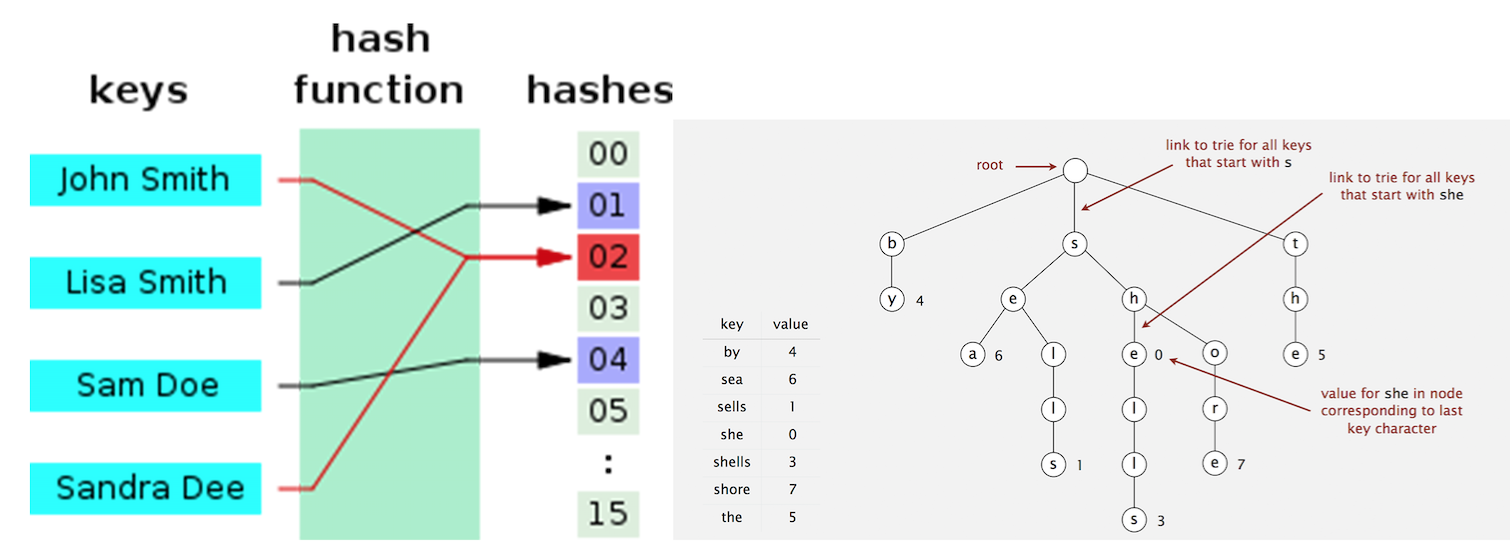
\includegraphics[width=0.8\textwidth]{images/hashing.png}
    \caption{Software Architecture Diagram}
    \label{fig:software_architecture}
\end{figure}

\subsection{Communication Interfaces}
The system will utilize HTTP and WebSocket protocols for communication between components. Table~\ref{tab:communication_interfaces} lists the communication protocols.

\begin{table}[h]
    \centering
    \begin{tabular}{|l|l|}
        \hline
        \textbf{Protocol} & \textbf{Usage} \\ \hline
        HTTP & Standard API communication \\ \hline
        WebSocket & Real-time updates \\ \hline
    \end{tabular}
    \caption{Communication Interfaces}
    \label{tab:communication_interfaces}
\end{table}

\section{Functional Requirements}
The functional requirements specify the system's behavior.

\subsection{Use Case}
Below is an example use case for user login:

\begin{table}[h]
    \centering
    \begin{tabular}{|l|l|}
        \hline
        \textbf{Use Case ID} & UC001 \\ \hline
        \textbf{Use Case Name} & User Login \\ \hline
        \textbf{Description} & Allows users to log into the system \\ \hline
        \textbf{Actors} & End User \\ \hline
        \textbf{Preconditions} & User has valid credentials \\ \hline
        \textbf{Postconditions} & User is logged in \\ \hline
    \end{tabular}
    \caption{Use Case Example}
    \label{tab:use_case}
\end{table}

\subsection{Use Case Diagram}
An example use case diagram is shown in Figure~\ref{fig:use_case_diagram}.

\begin{figure}[h]
    \centering
    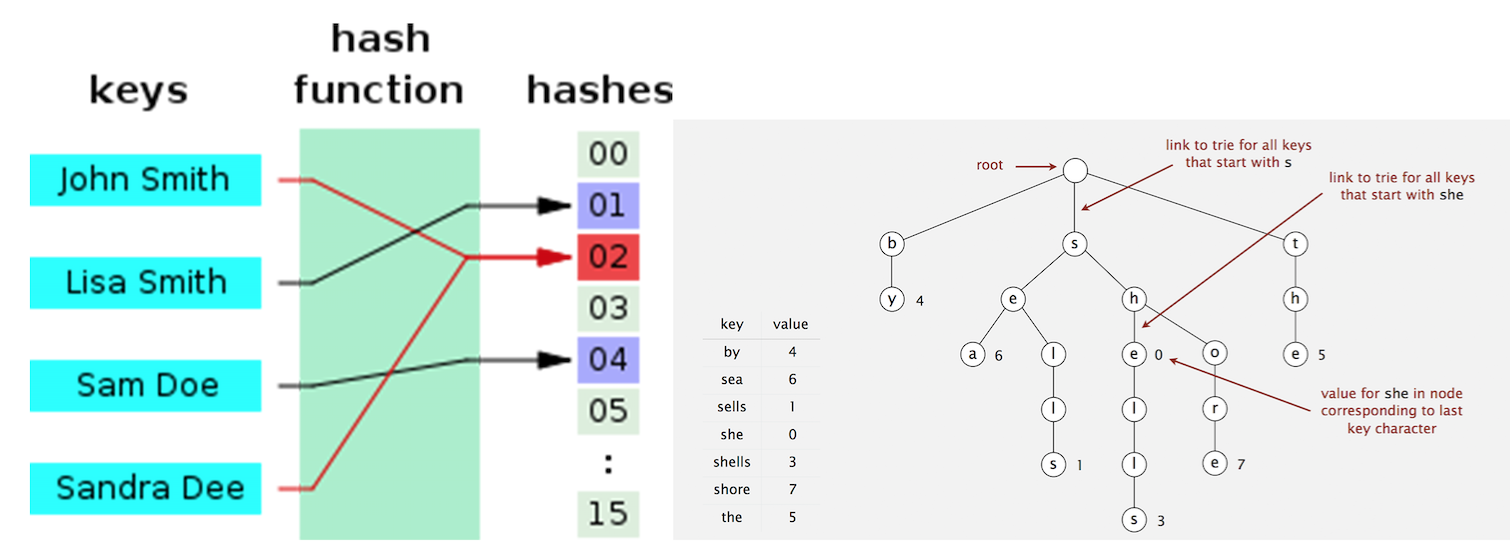
\includegraphics[width=0.7\textwidth]{images/hashing.png}
    \caption{Use Case Diagram}
    \label{fig:use_case_diagram}
\end{figure}

\subsection{Data Dictionary}
The data dictionary defines key data elements in the system. Table~\ref{tab:data_dictionary} provides an example.

\begin{table}[h]
    \centering
    \begin{tabular}{|l|l|l|}
        \hline
        \textbf{Field Name} & \textbf{Data Type} & \textbf{Description} \\ \hline
        UserID & Integer & Unique identifier for each user \\ \hline
        Username & String & User's login name \\ \hline
        PasswordHash & String & Encrypted user password \\ \hline
    \end{tabular}
    \caption{Data Dictionary Example}
    \label{tab:data_dictionary}
\end{table}

\section{Non-functional Requirements}

\subsection{Product Requirements}
The system must meet performance benchmarks. Table~\ref{tab:performance_requirements} highlights key metrics.

\begin{table}[h]
    \centering
    \begin{tabular}{|l|l|}
        \hline
        \textbf{Metric} & \textbf{Requirement} \\ \hline
        Response Time & Less than 200ms for 95\% of requests \\ \hline
        Uptime & 99.9\% availability \\ \hline
        Scalability & Support up to 10,000 concurrent users \\ \hline
    \end{tabular}
    \caption{Performance Requirements}
    \label{tab:performance_requirements}
\end{table}

\section{API Specifications}
Figure~\ref{fig:api_interaction} illustrates the interaction between different APIs.

\begin{figure}[h]
    \centering
    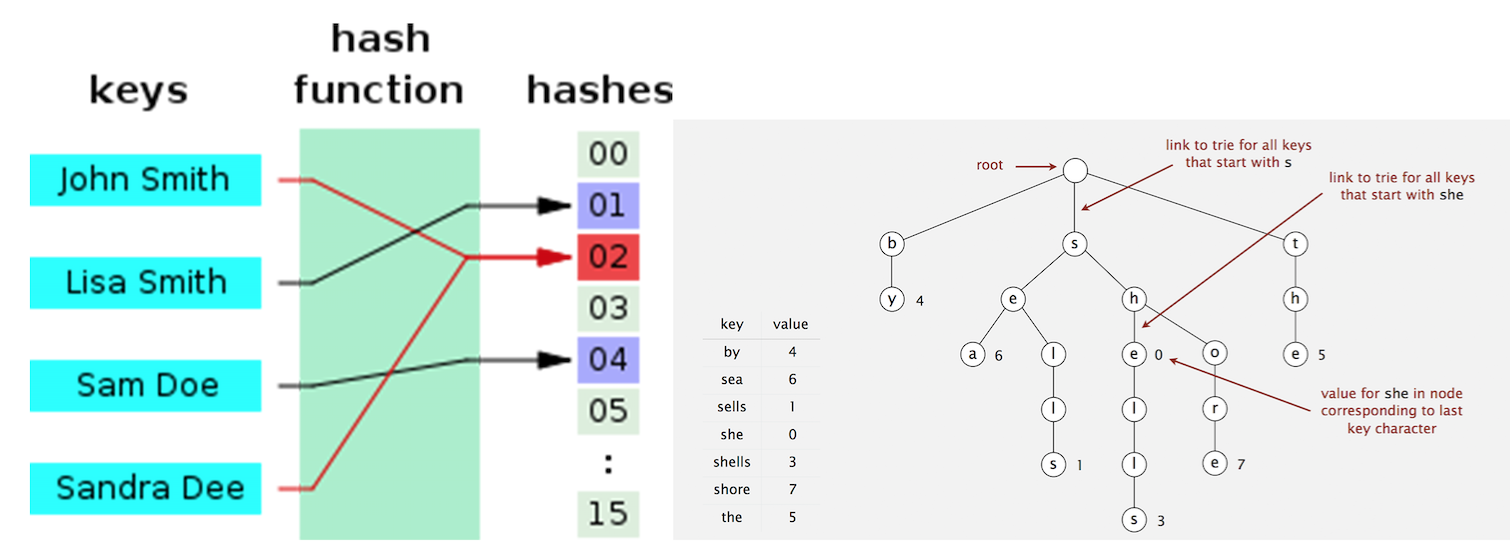
\includegraphics[width=0.9\textwidth]{images/hashing.png}
    \caption{API Interaction Diagram}
    \label{fig:api_interaction}
\end{figure}

\section{Main Chain Architecture}
The main chain architecture, as illustrated in Figure~\ref{fig:main_chain}, shows the core workflow.

\begin{figure}[h]
    \centering
    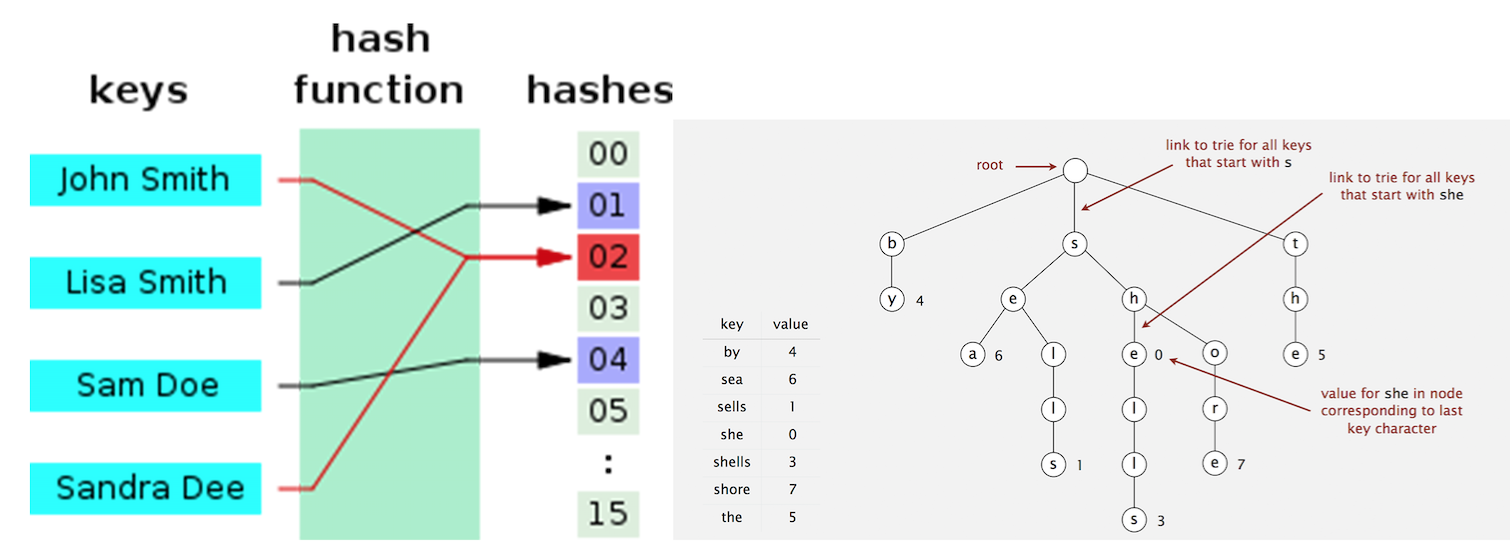
\includegraphics[width=0.8\textwidth]{images/hashing.png}
    \caption{Main Chain Architecture}
    \label{fig:main_chain}
\end{figure}

\section{Database Architecture}
The database schema is presented in Figure~\ref{fig:database_schema}.

\begin{figure}[h]
    \centering
    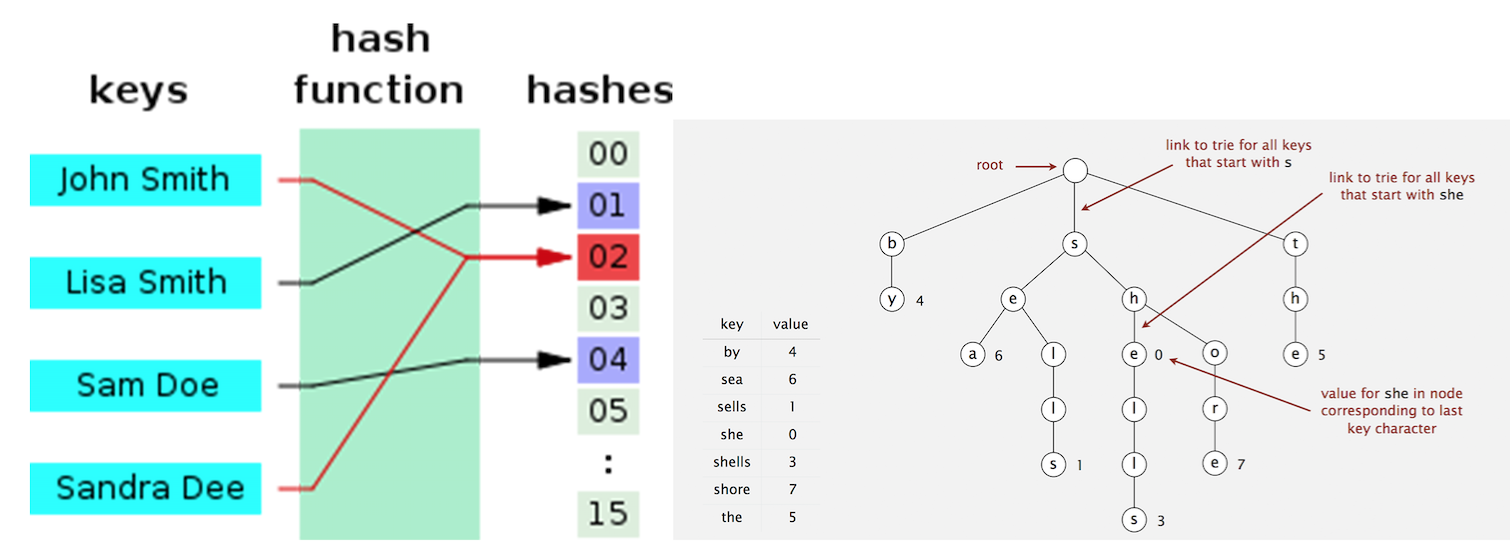
\includegraphics[width=0.8\textwidth]{images/hashing.png}
    \caption{Database Schema}
    \label{fig:database_schema}
\end{figure}

\section{System Evolution}
\subsection{Limitation and Assumption}
The system assumes constant network availability, which may limit usage in offline environments.

\subsection{Anticipated Changes}
Future updates will include machine learning capabilities for enhanced predictions.
